\chapter{Implementazione e test}
\label{chap:implTest}

\begin{minipage}{12cm}\textit{In questo capitolo si illustreranno gli aspetti tecnici relativi alla realizzazione del software: la scelta delle librerie e dell'ambiente di sviluppo, i problemi riscontrati e le soluzioni intraprese. Si procederà inoltre alla validazione del sistema e la valutazione delle prestazioni.}
\end{minipage}

\vspace*{1cm}

\section{Lo sviluppo}
\label{sec:sviluppo}
Nei precedenti capitoli si è discusso principalmente degli strumenti teorici che, come spesso segnalato, sono stati selezionati o sintetizzati con in mente il requisito di efficienza imprescindibile in un contesto di controllo nel quale ci si pone. Sono stati selezionati perciò gli algoritmi migliori rispetto ad un rapporto efficacia/costo computazionale. Inoltre, si sono scelti quelli meglio parallelizzabili su architetture vettorizzate o dotate di co-processori grafici. Nel seguito verrà descritto l'aspetto implementativo del software Visual Observer. Si descriveranno in particolare gli strumenti di sviluppo, le librerie usate e l'architettura software implementata. 

\subsection{Ambiente di sviluppo e target}
\label{sec:dev:ambiente}

Prima di poter scrivere anche una sola linea di codice, si deve aver ben chiaro l'obbiettivo di sviluppo che ci si pone al fine di poter valutare quale può essere l'ambiente di sviluppo, il linguaggio e le librerie da utilizzare.  Conviene allora specificare e definire i requisiti di progetto:
\begin{itemize}
	\item \textbf{Architettura target:}  x86\_64, ARM,
	\item \textbf{Sistema Operativo target:}  Windows, GNU/Linux,
	\item \textbf{Specifiche hardware minime:}
	\begin{itemize}
		\item CPU: x86\_64 o ARM,
		\item GPU: nessuna o generica con supporto OpenCL,
	\end{itemize} 
	\item \textbf{Specifiche hardware consigliate:}
		\begin{itemize}
			\item CPU: x86\_64 o ARM con supporto OpenCL o SIMD/AVX,
			\item GPU: coprocessore grafico NVidia ad alte prestazioni con supporto CUDA Shared Model $\ge$ 2.1,
		\end{itemize}			 
\end{itemize}

La scelta delle architetture e dei sistemi operativi non è casuale, ovviamente. Infatti, il supporto x86\_64 permette di poter sviluppare e testare il codice su un normale PC in ambiente Windows o Linux. D'altro canto il software è pensato per essere utilizzato a bordo di un sistema di controllo di un robot e tipicamente quest'ultimi hanno processori ARM su sistema Linux.

Spesso si è fatto riferimento nei capitoli precedenti ad un requisito di esecuzione real-time. Formalmente esso è difficile da definire, si può intendere però nel seguente modo: \textit{si fissi una piattaforma hardware abbastanza potente, si richiede che il tempo di esecuzione del software di stima sia tale da rendere la stessa disponibile in tempo utile.} Ad esempio, si potrebbe richiedere che su una scheda di sviluppo Nvidia TX1, dotata delle specifiche di cui sopra, sia in grado si fornire una stima con frequenza 15 Hz o superiore.
 
Si può comprendere allora la specifica richiesta della presenza di un processore vettorizzato o un coprocessore grafico con supporto a OpenCL o CUDA. Infatti, in questi casi è possibile ridurre di moltissimo i tempi di esecuzione grazie alla parallelizzazione dei calcoli.

Alla luce di quanto su detto, la scelta del linguaggio di sviluppo è ricaduta sul \textbf{C++}. Infatti esso permette di ottenere un codice macchina particolarmente ottimizzato e al contempo di mantenere la portabilità dello stesso. Il codice è stato sviluppato utilizzando il sistema operativo \textbf{Windows} e l'ambiente di sviluppo \textbf{Visual Studio Community 2015}. Tale scelta è motivata da diversi fattori:
\begin{enumerate}
	\item Allo stato attuale, Visual Studio permette di sviluppare e compilare codice, in modo semplice, per tutti i sistemi operativi e le architetture su citati.
	\item In ambiente Linux non si sarebbe potuto sviluppare per Windows.
	\item Rende lo sviluppo più semplice e veloce, grazie anche a numerosi strumenti di debug e profiling messi a disposizione.
	\item Per scopi accademici (e piccoli progetti commerciali) è distribuito gratuitamente.
\end{enumerate}

Nel seguito si presenta una breve descrizione delle librerie software utilizzate: OpenCV e CUDA. Non si farà riferimento a OpenCL perché non direttamente utilizzata. Infatti, grazie all'uso di OpenCV l'utilizzo della stessa o di un altro sistema di vettorizzazione è del tutto trasparente. Come sarà chiaro più avanti nel paragrafo dedicato al testing, l'attivazione o meno di quest'ultima però darà luogo a prestazioni nettamente superiori. Informalmente, OpenCL è un architettura hardware e software per il calcolo parallelo. Essa permette di utilizzare sia CPU che GPU (anche Nvidia), talvolta in contemporanea, per effettuare calcoli generici.

\subsection{OpenCV}
\label{sec:tools:opencv}

OpenCV, acronimo in lingua inglese di \textbf{Open} source \textbf{C}omputer \textbf{V}ision library, è una libreria software multi piattaforma per la visione artificiale. Essa nella sua prima versione risale al lontano 2000 ed è stata originariamente sviluppata ad opera di Intel. Successivamente il progetto è stato preso in carico dalla comunità open source ed è mantenuto da un numero elevato di appassionati e sviluppatori. Oggi giorno, è considerata lo standard di fatto utilizzato per progetti comprendenti la visione artificiale in progetti sia accademici che commerciali. Essa comprende molteplici ambiti tra cui: calcolo matriciale e strumenti di algebra lineare, riconoscimento delle feature, stereoscopia e filtraggio delle immagini. Di giorno in giorno gli strumenti presenti vengono ottimizzati e di nuovi ne vengono aggiunti. 
La libreria è scritta principalmente in codice C++, fortemente ottimizzato per sfruttare le particolarità della piattaforma target: vettorizzazione SIMD e AVX, openCL, CUDA. Risulta perciò un valido strumento in progetti di applicazioni real-time. Esistono poi numerosi wrapper che permettono il suo impiego in altri linguaggi tra cui: Python, Java, C\#. Inoltre è disponibile per praticamente tutti i maggiori sistemi operativi: Windows, Linux, Android, IOs e OsX e per le maggiori architetture: x86, x86\_64, ARM.
Infine si segnala che è rilasciata sotto licenza BSD perciò può essere liberamente impiagata in progetti sia accademici che commerciali.

\subsection{CUDA}
\label{sec:tools:cuda}
CUDA (acronimo di Compute Unified Device Architecture) è un'architettura hardware per l'elaborazione parallela creata da NVIDIA. Essa, unitamente all'ambiente di sviluppo CUDA, permette scrivere applicazioni capaci di eseguire calcolo parallelo sulle GPU Nvidia. I linguaggi di programmazione disponibili nell'ambiente di sviluppo per CUDA, sono estensioni dei linguaggi più diffusi per scrivere programmi. Il principale è "CUDA-C" (C con estensioni NVIDIA), altri sono estensioni di Python, Fortran, Java e MATLAB.

Diversamente dalle CPU, le GPU hanno un'architettura parallela con diversi core, ognuno capace di eseguire centinaia di processi simultaneamente, se un'applicazione è adatta per quel tipo di architettura la GPU può offrire grandi prestazioni e benefici. Questo approccio di risoluzione dei problemi è noto come GPGPU (General Purpose GPU). In generale un ottimo contesto di esecuzione per questo tipo di dispositivi è quando vengono avviati moltissimi thread con lo stesso flusso di esecuzione. In realtà infatti le GPU estremizzano il concetto di vettorizzazione. Si hanno a disposizione un certo numero di Shared Processor, capaci di eseguire un gruppo di thread alla volta detto Warp. Per poter eseguire un Warp in modo parallelo deve accadere che tutti i thread che lo compongono eseguano le stesse operazioni, ovviamente su indirizzi di memoria differenti. Inoltre per rendere gli accessi in memoria efficienti e ridurre (anche drasticamente) i tempi di calcolo i thread devono poter accedere alla memoria in modo adatto. Infatti, le GPU gestiscono la memoria in modo opposto rispetto alle CPU, cioè locazioni di memoria vicine sono disposte in diversi banchi di memoria. Il motivo di tale scelta risiede nel fatto che le richieste in memoria sono solitamente molto lente e si cerca di parallelizzare la lettura in memoria al fine di rendere i dati disponibili simultaneamente per tutti i thread di un Warp. 

Alla luce di ciò, è chiaro che non tutte le applicazioni possono essere parallelizzate su coprocessore grafico ed è inoltre chiaro perché un forte accento si è posto sul trovare algoritmi parallelizzabili. Ad esempio questo è il caso del comparatore a forza bruta, presentato nel paragrafo \ref{sec:det:bmmatch}, che seppur utilizza un approccio poco intelligente risulta molto veloce.

\subsection{L'architettura software}
\label{sec:dev:arch}
Infine, per concludere il paragrafo, si presenta l'architettura software sviluppata. Essa è pensata per essere completamente modulare ed intercambiabile. I blocchi funzionali contraddistinti con la lettera "I" maiuscola sono delle interfacce e diverse implementazioni ne sono fornite.
\begin{figure}[h!]
	\centering
	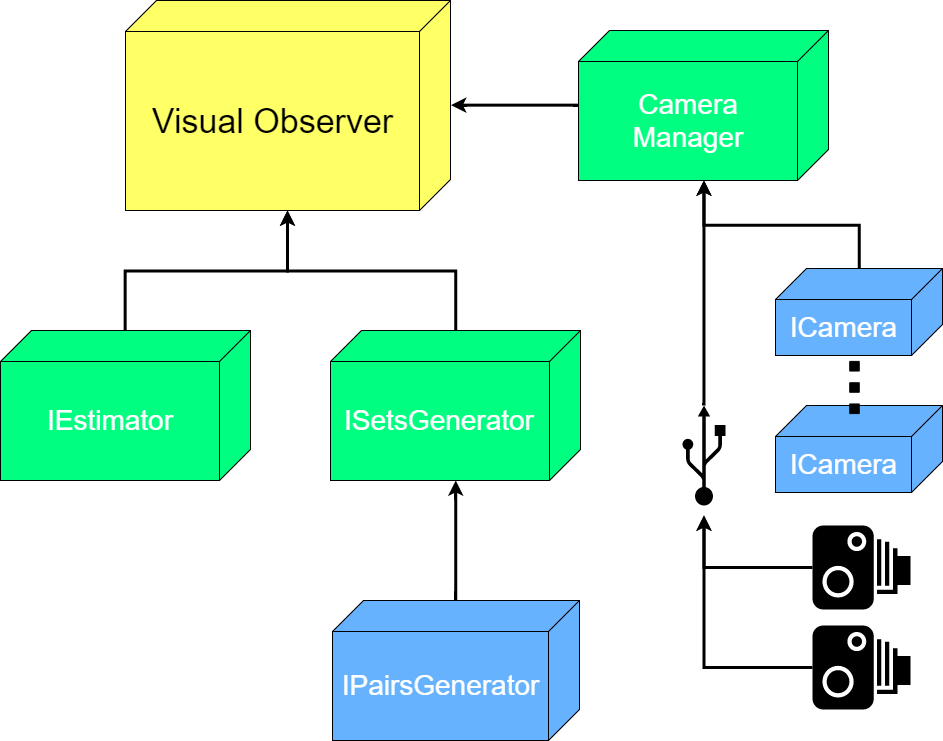
\includegraphics[width=400pt]{imgs/arch.png}
	\caption{Rappresentazione architettura software Visual Observer.}
	\label{vis:impl:arch}
\end{figure} 

L'architettura inoltre prevede che essi possano essere sostituiti da future implementazioni. 

\section{Validazione e test}
\label{sec:test}

\subsection{Il motore grafico Unity3D}
\label{sec:unity}

\subsection{Vantaggi e svantaggi di una validazione con motore grafico}
\label{sec:valid}

\subsection{Risultati ottenuti}
\label{sec:perf}